\documentclass{beamer}
%\usepackage{xspace}
\usepackage{amsmath,amssymb}
\usepackage{graphicx}
%\usepackage{svg}
%\usepackage{pgfpages}
%\pgfpagesuselayout{4 on 1}[a4paper,border shrink=5mm,landscape]
%\usepackage{psfrag}
%\usepackage[usenames,dvipsnames]{xcolor}
\usepackage{braket}
\usepackage{tikz}
\usetikzlibrary{graphs}
\usetikzlibrary{datavisualization}
\usetikzlibrary{datavisualization.formats.functions}
\usepackage{pgfplotstable}
\usepgfplotslibrary{patchplots}

\setbeamercovered{transparent}

\usetheme{Pittsburgh}
%\usetheme{default}

\setbeamertemplate{sidebar right}{}
\setbeamertemplate{footline}[frame number]
%\usefonttheme{professionalfonts}

%\usepackage{sansmathaccent}
%\usepackage{bm}

%\usepackage{unicode-math}
%%\setmainfont[SlantedFont={Latin Modern Roman Slanted},SlantedFeatures={Color=000000},
%%  SmallCapsFont={TeX Gyre Termes},SmallCapsFeatures={Letters=SmallCaps}]{XITS}
%\setmathfont[math-style=ISO,sans-style=upright]{XITS Math}
%\setmathfont[range={\mathcal,\mathbfcal}]{Latin Modern Math}

\usepackage{sfmath}

%\mathversion{sans}

\newcommand{\Tr}{\mathsf{Tr}}

\definecolor{redorange}{rgb}{1.0, .25, .25}
\definecolor{citation}{rgb}{.1, 0.8, .35}
\newcommand\emm[1]{\textcolor{redorange}{{#1}}}
\newcommand\numc[1]{\textcolor{citation}{{\bf #1}}}

%\newcommand\bm[1]{{\mbox{\boldmath $#1$}}}
\newcommand\bm[1]{{\mathbf{#1}}}
%\newcommand\bm[1]{{\bf #1}}
%\newcommand\bm[1]{\ensuremath{\boldsymbol{#1}}}
%\newcommand\bm[1]{{\textbf{\it #1}}}

\title{A single qubit}
\author{Ryuhei Mori}
%\institute{$\vcenter{\hbox{\includegraphics[width=30pt]{ELC_logo}}}$ Postdoctoral Fellow of ELC\\ $\vcenter{\hbox{\includegraphics[width=20pt]{titech_logo}}}$ Tokyo Institute of Technology}
\institute{Tokyo Institute of Technology}
%\date{21, Feb, 2019}



\begin{document}
\begin{frame}[plain]
\maketitle
\end{frame}

\begin{frame}{Operation in a system}
We will manipulate quantum state.

\vspace{2em}
This operation can be represented by a map $T: \text{Set of states} \to \text{Set of states}$.

\vspace{2em}
\end{frame}

\begin{frame}{A single bit}
\begin{itemize}
\setlength{\itemsep}{2em}
%\item State: \texttt{0},  \texttt{1} and their probabilistic mixture.
%\item Binary measurement: \texttt{0?}, \texttt{1?} and ther linear combination with coefficients in $[0,1]$.
\item 
%\begin{equation*}
$\text{Set of states} = \left\{\omega\in\mathbb{R}^2 \mid \omega\in C_{\ge 0}, \langle u, \omega\rangle = 1\right\}$.
%\end{equation*}
\item 
%\begin{equation*}
$\text{\small Set of binary measurements} = \left\{e\in\mathbb{R}^2 \mid e\in C_{\ge 0}, u-e \in C_{\ge 0} \right\}$.
%\end{equation*}
\end{itemize}

\vspace{1em}
\centering
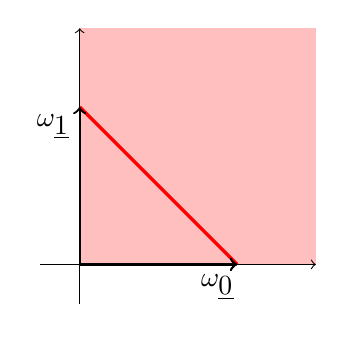
\begin{tikzpicture}
\draw[pink, fill] (0,0) rectangle +(3,3);
\draw[->] (-0.5,0) -- (3,0);
\draw[->] (0,-0.5) -- (0,3);
\draw[very thick, red] (2,0) -- (0,2);
\draw[->, thick] (0,0) -- node[anchor=north, very near end] {$\omega_{\underbar{0}}$} (2,0);
\draw[->, thick] (0,0) -- node[anchor=east, very near end] {$\omega_{\underbar{1}}$} (0,2);
\draw[->, thick] (0,0) -- (2,0);
\end{tikzpicture}
\hfill
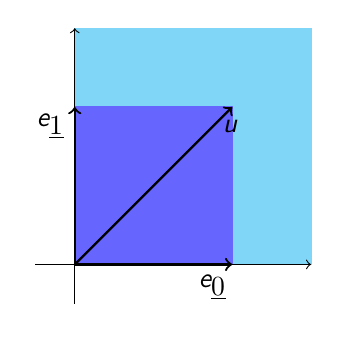
\begin{tikzpicture}
\draw[cyan!50, fill] (0,0) rectangle +(3,3);
\draw[blue!60, fill] (0,0) rectangle +(2,2);
\draw[->] (-0.5,0) -- (3,0);
\draw[->] (0,-0.5) -- (0,3);
%\draw (0,0) -- (2,2);
\draw[->, thick] (0,0) -- node[anchor=north, very near end] {$e_{\underbar{0}}$} (2,0);
\draw[->, thick] (0,0) -- node[anchor=east, very near end] {$e_{\underbar{1}}$} (0,2);
\draw[->, thick] (0,0) -- node[anchor=west, very near end] {$u$} (2,2);
\end{tikzpicture}

%Operation
%\begin{itemize}
%\item Identity: \texttt{0} $\mapsto$ \texttt{0}, \texttt{1} $\mapsto$ \texttt{1}
%\item Bit flip: \texttt{0} $\mapsto$ \texttt{1}, \texttt{1} $\mapsto$ \texttt{0}
%\end{itemize}
\end{frame}

\begin{frame}{A single qubit}
\begin{itemize}
\setlength{\itemsep}{3em}
\item State: A $2\times 2$ Hermitian matrix $\rho$ satisfying $\rho\succeq0$ and $\Tr(\rho)=1$.
\item Binary measurements: A $2\times 2$ Hermitian matrix $\rho$ satisfying $\rho\succeq0$ and $I-\rho\succeq0$.
\end{itemize}
\end{frame}

\begin{frame}{A single qubit}
\begin{itemize}
\setlength{\itemsep}{3em}
\item A qubit can be represented by
\begin{equation*}
\rho = \frac12\left(I + r_x X + r_y Y + r_z Z\right)
\end{equation*}
for $[r_x\, r_y\, r_z]\in\mathbb{R}^3$ satisfying $r_x^2+r_y^2+r_z^2\le 1$.
\item A qubit can be represented by a point $[r_x\,r_y\,r_z]$ in a three-dimensional sphere of radius 1.
\end{itemize}
\end{frame}

\begin{frame}{Bloch sphere}
\end{frame}

\begin{frame}{Spectral decomposition of Hermitian matrix}
\end{frame}

\begin{frame}{Pauli matrices}
\begin{itemize}
\setlength{\itemsep}{3em}
\item 
\begin{equation*}
Z=\begin{bmatrix}1&0\\0&-1\end{bmatrix}=
\begin{bmatrix}1\\0\end{bmatrix}\begin{bmatrix}1&0\end{bmatrix}
-\begin{bmatrix}0\\1\end{bmatrix}\begin{bmatrix}0&1\end{bmatrix}
\end{equation*}
\item 
\begin{equation*}
X=\begin{bmatrix}0&1\\1&0\end{bmatrix}=
\frac12\begin{bmatrix}1\\1\end{bmatrix}\begin{bmatrix}1&1\end{bmatrix}
-\frac12\begin{bmatrix}1\\-1\end{bmatrix}\begin{bmatrix}1&-1\end{bmatrix}
\end{equation*}
\item 
\begin{equation*}
Y=\begin{bmatrix}0&-i\\i&0\end{bmatrix}=
\frac12\begin{bmatrix}1\\i\end{bmatrix}\begin{bmatrix}1&-i\end{bmatrix}
-\frac12\begin{bmatrix}1\\-i\end{bmatrix}\begin{bmatrix}1&i\end{bmatrix}
\end{equation*}
\end{itemize}
\end{frame}

\begin{frame}{Braket notation}
\begin{align*}
\ket{0} &:= \begin{bmatrix}1\\0\end{bmatrix},&
\ket{1} &:= \begin{bmatrix}0\\1\end{bmatrix}
\end{align*}
\begin{align*}
\ket{+} &:= \frac1{\sqrt{2}}\begin{bmatrix}1\\1\end{bmatrix},&
\ket{-} &:= \frac1{\sqrt{2}}\begin{bmatrix}1\\1\end{bmatrix}\\
&=\frac1{\sqrt{2}}(\ket{0}+\ket{1}),&
&=\frac1{\sqrt{2}}(\ket{0}0\ket{1})
\end{align*}
\begin{align*}
\ket{\psi} = \alpha\ket{0}+\beta\ket{1}
\end{align*}
for $|\alpha|^2+|\beta|^2=1$.
\end{frame}

\begin{frame}{Special states}
\end{frame}

\begin{frame}{State vector and unitary transform}
\end{frame}

\end{document}
